\documentclass{jsarticle}
\usepackage[dvipdfmx]{graphicx}
\usepackage{listings}
\usepackage{afterpage}
\begin{document}
\title{課題6 画像の2値化}
\author{13EC060 武澤 裕介}
\maketitle
\begin{abstract}
まずmatlabを用いてしきい値設定による単なる2値化をした後、ディザ法による2値化を行い考察する。
\end{abstract}
\section{2値化}
まず、今回使用する原画像を図1に示す。


\begin{figure}[htbp]
 \begin{center}
  
\includegraphics[width=5cm,height=5cm]{index.jpg}
 \end{center}
 \caption{原画像}
\end{figure}

\begin{lstlisting}[basicstyle=\ttfamily\footnotesize, frame=single]
filename = uigetfile('*');
ORG=imread(filename); % 原画像の入力
ORG = rgb2gray(ORG); colormap(gray); colorbar;
imagesc(ORG); axis image; % 画像の表示
pause; % 一時停止
 \end{lstlisting}
を用いてまず入力画像のグレースケール画像を表示させる。

\newpage
\begin{figure}[htbp]
 \begin{center}
  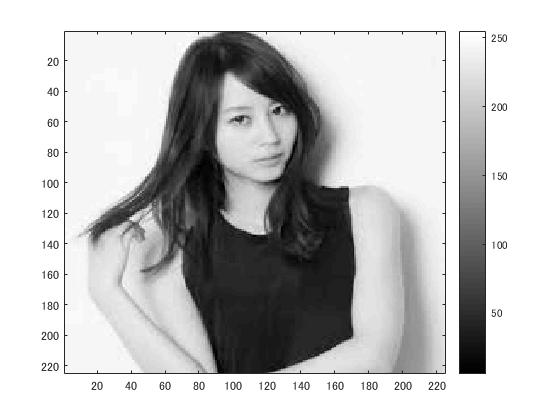
\includegraphics[width=10cm]{kadai6-0.jpg}
 \end{center}
 \caption{グレースケール画像}
\end{figure}

次に
\begin{lstlisting}[basicstyle=\ttfamily\footnotesize, frame=single]
IMG = ORG>128; % 128による二値化
imagesc(IMG); colormap(gray); colorbar; % 画像の表示
pause;
 \end{lstlisting}
を用いてしきい値128で単なる2値化を行う。

\newpage
\begin{figure}[htbp]
 \begin{center}
  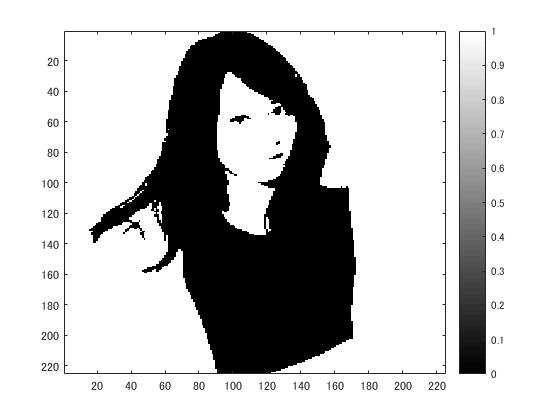
\includegraphics[width=10cm]{kadai6-1.jpg}
 \end{center}
 \caption{単純な2値化}
\end{figure}

最後に
\begin{lstlisting}[basicstyle=\ttfamily\footnotesize, frame=single]
IIMG = dither(ORG); % ディザ法による二値化
imagesc(IMG); colormap(gray); colorbar; % 画像の表示
 \end{lstlisting}
を用いてディザ法による2値化を行う。

\newpage
\begin{figure}[htbp]
 \begin{center}
  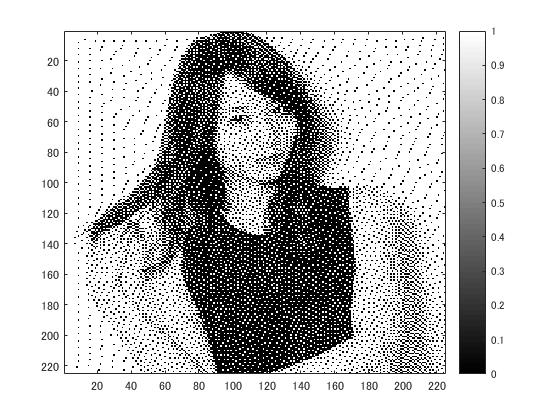
\includegraphics[width=10cm]{kadai6-2.jpg}
 \end{center}
 \caption{ディザ法による2値化}
\end{figure}


\section{考察}
今回単純な2値化とディザ法による2値化を行った。単なる2値化はしきい値に従った一般的な2値化であったが、ディザ法による2値化は目の錯覚によって2値化であるのに濃淡が見られるように見えた。

\end{document}